\documentclass[aspectratio=169, t, 8pt]{beamer}

%------configurando acentos-----------
\usepackage[utf8]{inputenc}
\usepackage[T1]{fontenc}
\usepackage[brazilian]{babel}
\usepackage{montserrat}
\usefonttheme[onlymath]{serif}
\usepackage{booktabs} % Tabelas elegantes sem linhas verticais
\usepackage{multirow}
\usepackage{array}
\usepackage[most]{tcolorbox}
\usepackage{graphicx}
\usepackage{xcolor}
\usepackage{colortbl}
\usepackage{ulem}
\usepackage{enumitem}

\DeclareMathOperator{\sen}{sen}
\DeclareMathOperator{\coss}{cos}
\DeclareMathOperator{\tg}{tg}
%-------Estilos Beamer---------------
\usetheme{metropolis}
%\usecolortheme{crane}
%\usefonttheme{serif}
\linespread{1.2}

% Personalização de Cores (Exemplo: Minimal Teal)
% Cores Base
\definecolor{BgCanvas}{HTML}{F9F9FB}      % Off-white muito suave
\definecolor{MainText}{HTML}{2B2D42}      % Grafite escuro para alta legibilidade
\definecolor{PrimaryAccent}{HTML}{4A6FA5} % Azul poeira (Dusty Blue)

% Tons Pastéis para Destaques e Cards
\definecolor{PastelGreenBg}{HTML}{E8F0EC}  % Sálvia Claro (Sucesso / Destaque Positivo)
\definecolor{PastelGreenFg}{HTML}{2D5A44}

\definecolor{PastelCoralBg}{HTML}{FDEAE6}  % Coral Soft (Atenção / Problema / Alerta)
\definecolor{PastelCoralFg}{HTML}{7A3025}

\definecolor{PastelPurpleBg}{HTML}{F0EBF4} % Lavanda (Conceitos / Citações)
\definecolor{PastelPurpleFg}{HTML}{4A3E56}

\definecolor{PastelYellowBg}{HTML}{FFF4E6} % Areia / Manteiga (Notas / Dados Secundários)
\definecolor{PastelYellowFg}{HTML}{7A522A}

% --- CONFIGURAÇÕES DE TEMA BEAMER ---
%\usetheme{metropolis}

\setbeamertemplate{itemize item}{\textcolor{MainText}{$\bullet$}}
\setbeamertemplate{itemize subitem}{\textcolor{MainText}{\scriptsize$\circ$}}
\setbeamertemplate{itemize 3rditem}{\textcolor{MainText}{\tiny$\blacksquare$}}

\setbeamercolor{background canvas}{bg=BgCanvas}
\setbeamercolor{normal text}{fg=MainText}
\setbeamercolor{frametitle}{bg=PastelGreenFg, fg=BgCanvas}
\setbeamercolor{title}{fg=MainText}
\setbeamercolor{subtitle}{fg=PrimaryAccent}
\setbeamercolor{structure}{fg=PrimaryAccent}

% Remove a linha amarela padrão do Metropolis sob o título
\setbeamertemplate{title separator}{}
\setbeamertemplate{progress bar in section page}{}

% ==============================================================================
% PALETA DE CORES "GEOMETRIA AQUECIDA" (Inspirada na imagem)
% ==============================================================================
\definecolor{BgCream}{HTML}{FFFDFB}       % Fundo creme suave
\definecolor{TextDark}{HTML}{2C1A14}      % Texto em castanho escuro elegante
\definecolor{PrimaryOrange}{HTML}{E0531C}  % Laranja vibrante (Títulos e destaques)
\definecolor{Terracotta}{HTML}{B8380D}     % Terracota queimado (Alertas)
\definecolor{SoftOrange}{HTML}{FFE6D5}     % Laranja bem suave (Fundo de blocos)

% =================================================
% CONFIGURAÇÃO DO TEMA METROPOLIS
% =================================================
% Cores do texto e fundo geral
\setbeamercolor{normal text}{fg=TextDark, bg=BgCream}
\setbeamercolor{alerted text}{fg=Terracotta}
\setbeamercolor{example text}{fg=PrimaryOrange}

% Barra de título dos slides (Frametitle)
\setbeamercolor{frametitle}{fg=BgCream, bg=PrimaryOrange}

% Título principal da apresentação (Slide de Capa)
\setbeamercolor{titlelike}{fg=PrimaryOrange}
\setbeamercolor{subtitle}{fg=Terracotta}

% Barra de progresso (Linha do Metropolis)
\setbeamercolor{progress bar}{fg=PrimaryOrange, bg=PrimaryOrange!20}

% Customização de Blocos (block, alertblock, exampleblock)
\setbeamercolor{block title}{fg=BgCream, bg=PrimaryOrange}
\setbeamercolor{block body}{fg=TextDark, bg=SoftOrange}

\setbeamercolor{block title alerted}{fg=BgCream, bg=Terracotta}
\setbeamercolor{block body alerted}{fg=TextDark, bg=Terracotta!15}


% --- ESTILOS DE CARDS PASTEL COM TCOLORBOX ---
\newtcolorbox{cardPrincipal}[1][]{
  colback=SoftOrange,
  colframe=Terracotta,
  coltext=TextDark,
  arc=6pt,
  boxrule=0pt,
  left=12pt, right=12pt, top=10pt, bottom=10pt,
  fonttitle=\bfseries\small,
  #1
}

\newtcolorbox{cardcoral}[1][]{
  colback=PastelCoralBg,
  colframe=PastelCoralFg,
  coltext=PastelCoralFg,
  arc=6pt,
  boxrule=0pt,
  left=12pt, right=12pt, top=10pt, bottom=10pt,
  fonttitle=\bfseries\small,
  #1
}

\newtcolorbox{cardpurple}[1][]{
  colback=PastelPurpleBg,
  colframe=PastelPurpleFg,
  coltext=PastelPurpleFg,
  arc=6pt,
  boxrule=0pt,
  left=12pt, right=12pt, top=10pt, bottom=10pt,
  fonttitle=\bfseries\small,
  #1
}

\newtcolorbox{cardyellow}[1][]{
  colback=PastelYellowBg,
  colframe=PastelYellowFg,
  coltext=PastelYellowFg,
  arc=6pt,
  boxrule=0pt,
  left=12pt, right=12pt, top=10pt, bottom=10pt,
  fonttitle=\bfseries\small,
  #1
}

\graphicspath{{../../src/img/semana09/}}

%--------Dados do Documento
\title{Geometria Espacial: Poliedros, Esferas \& Visão 3D}
\subtitle{Relação de Euler, Secções Esféricas e Projeções Ortogonais}
\author{prof. Eduardo}
\institute{Pré-Universitário Oficina do Saber / UFF}

\date{\today}


%-------- Pacotes Matemática -------------
\usepackage{amsmath}
\usepackage{amsthm}
\usepackage{amsfonts}
\usepackage{amssymb}
\usepackage{xfrac}
\usepackage{thmtools}

\begin{document}

    \begin{frame} %capa
        \vspace*{\fill}
            
            \begin{columns}[c]
                \begin{column}{0.5\textwidth}
                    {\usebeamerfont{title}\usebeamercolor[fg]{title}\inserttitle}\vspace{0.2cm}
                    
                    {\usebeamerfont{subtitle}\usebeamercolor[fg]{subtitle}\insertsubtitle}\vspace{0.5cm}

                {\usebeamerfont{author}\insertauthor}\vspace{0.3cm}

                {\usebeamerfont{institute}\insertinstitute}\vspace{0.3cm}

                {\usebeamerfont{date}\insertdate}
            \end{column}
            
            
            \begin{column}{0.4\textwidth}
                \centering
                
\includegraphics[width=0.4\textwidth]{../logo_ofSaber.png}

                \vspace{.4cm}
                \vspace*{\fill}
        \begin{columns}[c]
            \begin{column}{.5\textwidth}
                \centering
\includegraphics[width=.5\textwidth]{../Proex02c.png}
            \end{column}
            \begin{column}{.5\textwidth}
                \centering
\includegraphics[width=0.4\textwidth]{../Logo_UFF.png}
            \end{column}
        \end{columns}
        \vspace*{\fill}
            \end{column}
        \end{columns}
    \vspace*{\fill}
    \end{frame}

    % \frame
        % {
        %     \usebackgroundtemplate{
        %     \includegraphics[width=\paperwidth]{segunda_capa_pitagoras.png}}
        %     \begin{frame}[plain]                
        %     \end{frame}
        % }

    \begin{frame}{Poliedros: Vértices, faces e arestas}
        \begin{columns}[totalwidth=.9\textwidth, T]
            \begin{column}{.45\textwidth}
                \begin{figure}
                    \centering
                    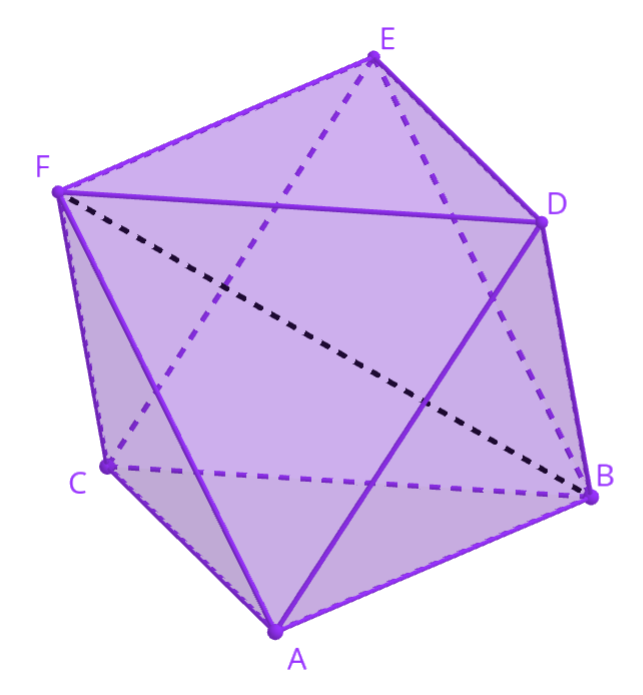
\includegraphics[width=.8\textwidth]{octaedro_segmento_interno.png}
                \end{figure}
            \end{column}

            \begin{column}{.45\textwidth}
                Um {\bf poliedro convexo} é um sólido limitado por polígonos planos, chamados de {\bf faces}. A união desses polígonos dá origem aos outros elementos que compõem o poliedro: {\bf arestas} e {\bf vértices}.

                \vspace{1.2em}

                Em um poliedro deste tipo, uma reta que una quaisquer dois pontos do poliedro estará contida no seu interior.

                \vspace{1.2em}

                {\large\bf Elementos de um poliedro convexo}

                \begin{itemize}
                    \item As \textit{faces} são os polígonos que delimitam o sólido (no exemplo, triângulos equiláteros);
                    \item As \textit{arestas} são os lados dos polígonos;
                    \item Os \textit{vértices} são os pontos em que as arestas se encontram
                \end{itemize}
            \end{column}
        \end{columns}
    \end{frame}

    \begin{frame}{Relação de Euler}
        \begin{columns}[totalwidth=0.9\textwidth]
            \begin{column}{.45\textwidth}
                \begin{figure}
                    \centering
                    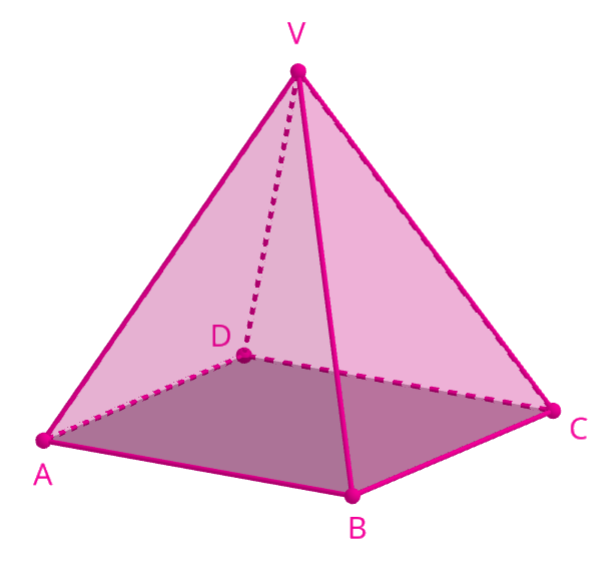
\includegraphics[width=.6\textwidth]{piramide_basequadrada.png}
                    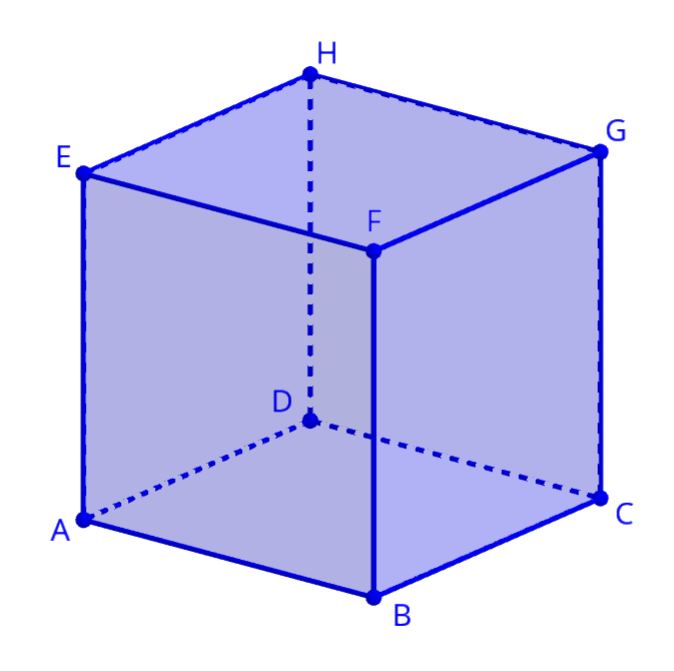
\includegraphics[width=.6\textwidth]{cubo.png}
                \end{figure}                
            \end{column}
            \begin{column}{.45\textwidth}
                A {\bf relação de Euler} é uma fórmula que relaciona o número de vértices, arestas e faces de um poliedro convexo. Essa relação é muito útil para contar elementos de um poliedro: dado o número de vértices e faces, podemos determinar o número de arestas, por exemplo.

                \vspace{1.2em}

                {\large\bf Relação de Euler}
                { \Large
                    \[
                        V - A + F = 2
                    \]
                }

                Onde:
                \begin{itemize}
                    \item $V$ é o número de vértices;
                    \item $A$ é o número de arestas;
                    \item $F$ é o número de faces.
                \end{itemize}
            \end{column}
        \end{columns}
    \end{frame}

    \begin{frame}{Contando Arestas}
        \begin{columns}[totalwidth=0.9\textwidth]
            \begin{column}{.45\textwidth}
                \begin{figure}
                    \centering
                    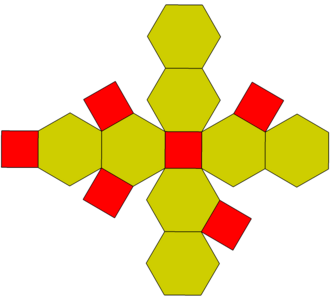
\includegraphics[width=.8\textwidth]{octaedro_truncado_planificacao.png}
                \end{figure}
            \end{column}
            \begin{column}{.45\textwidth}
                Questões que envolvem contagem de elementos de um poliedro nem sempre vão trazer de forma explícita o número de arestas. Nesses casos, podemos contar as arestas a partir do número de faces e do número de lados de cada face.

                \vspace{1.2em}

                Sabendo que cada aresta pertence a duas faces, podemos determinar o número de arestas de um poliedro convexo pela seguinte fórmula:

                \vspace{1.2em}

                {\large\bf Fórmula para contagem de arestas}
                { \Large
                    \[
                        A = \frac{F_1 \cdot n_1 + F_2 \cdot n_2 + F_3 \cdot n_3 + \cdots + F_i \cdot n_i}{2}
                    \]
                }
            \end{column}
        \end{columns}
    \end{frame}

    \begin{frame}{Sólidos de Platão}
        \begin{columns}[totalwidth=0.9\textwidth, T]
            \begin{column}{.45\textwidth}
                Os {\bf sólidos de Platão} são poliedros convexos que possuem faces congruentes e regulares, e o mesmo número de faces se encontram em cada vértice. Existem apenas cinco sólidos de Platão:

                \vspace{1.3 em}

                \setlength{\extrarowheight}{.4em}
                \begin{tabular}{ c c c }
                    \toprule
                    \bf Sólido & \bf Faces & \bf Vértices \\
                    \midrule
                    Tetraedro & 4 & 4 \\
                    \midrule
                    Cubo & 6 & 8 \\
                    \midrule
                    Octaedro & 8 & 6 \\
                    \midrule
                    Dodecaedro & 12 & 20 \\
                    \midrule
                    Icosaedro & 20 & 12 \\
                    \bottomrule
                \end{tabular}
            \end{column}

            \begin{column}{.4\textwidth}
                \centering
                \begin{tabular}{| c | c | c |}
                    \hline
                    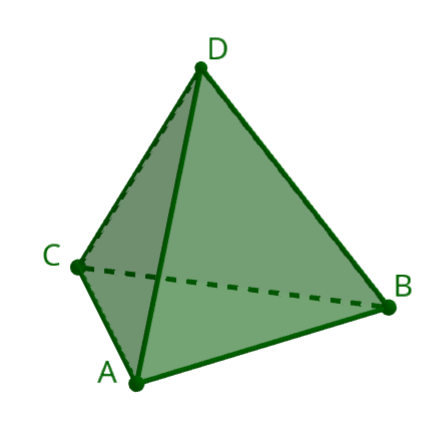
\includegraphics[width=.3\textwidth]{tetraedro.png} &
                    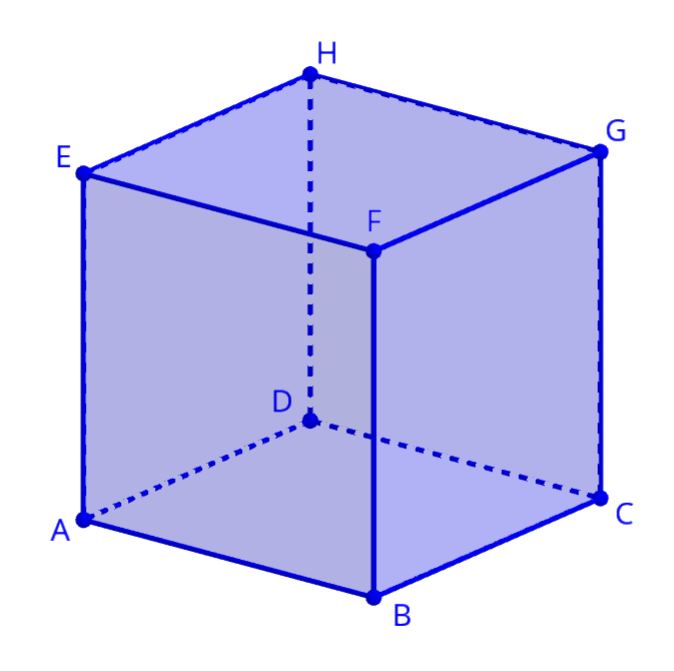
\includegraphics[width=.3\textwidth]{cubo.png} &
                    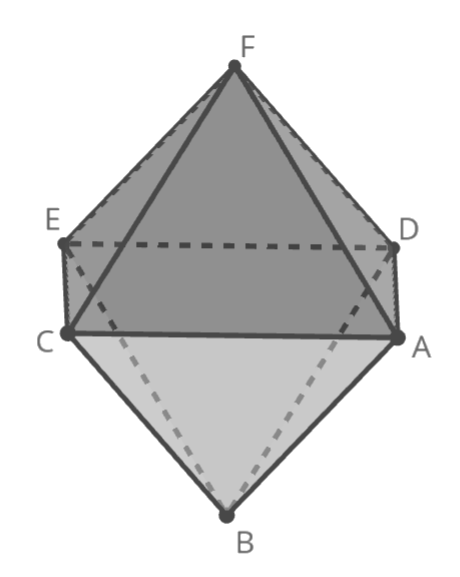
\includegraphics[width=.25\textwidth]{octaedro.png} \\
                    \hline
                    Tetraedro & Cubo & Octaedro \\
                    \hline
                \end{tabular}

                \vspace{1.2em}

                \begin{tabular}{|c|c|}
                    \hline
                    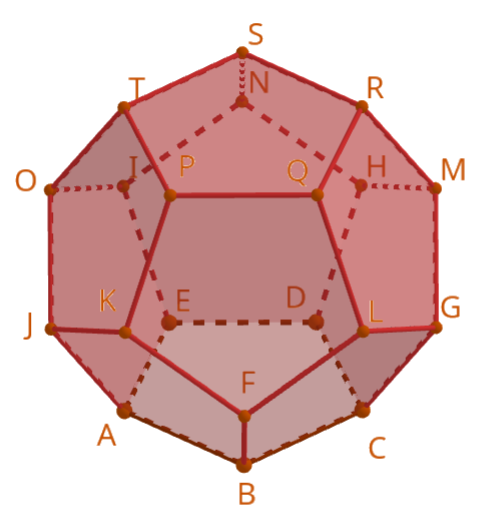
\includegraphics[width=.3\textwidth]{dodecaedro.png} &
                    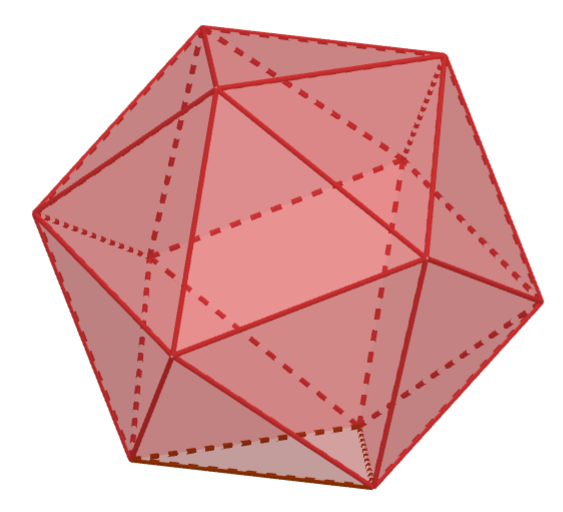
\includegraphics[width=.3\textwidth]{icosaedro.png} \\
                    \hline
                    Dodecaedro & Icosaedro \\
                    \hline
                \end{tabular}
                
            \end{column}
        \end{columns}
    \end{frame}

    \begin{frame}{Esferas}
        \begin{columns}[totalwidth=0.9\textwidth, T]
            \begin{column}{.45\textwidth}
                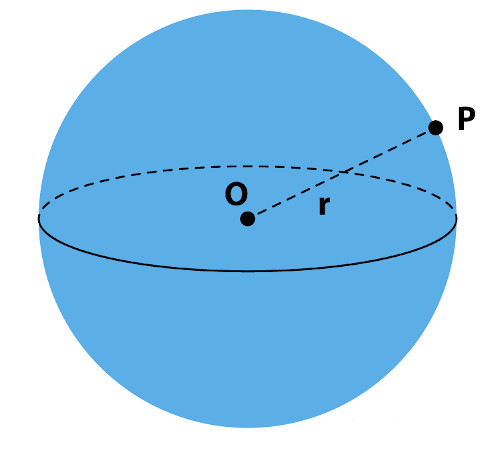
\includegraphics[width=.8\textwidth]{esfera.png}
            \end{column}
            \begin{column}{.45\textwidth}
                A {\bf esfera} é o conjunto de todos os pontos do espaço que estão a uma distância fixa de um ponto central. Essa distância fixa é chamada de {\bf raio} da esfera, e o ponto central é chamado de {\bf centro} da esfera. A esfera também pode ser definida pela rotação de um semicírculo em torno de um eixo que passa pelo seu centro.
            \end{column}
        \end{columns}
    \end{frame}

    \begin{frame}{Esfera: Volume}
        \begin{columns}[totalwidth=0.9\textwidth, T]
            \begin{column}{.45\textwidth}
                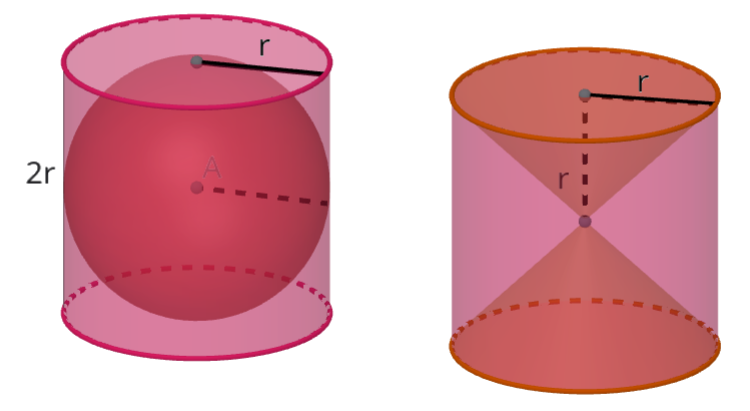
\includegraphics[width=\textwidth]{volume_esfera.png}
            \end{column}
            \begin{column}{.38\textwidth}
                O volume de uma esfera de raio $r$ é dado pela fórmula:
                
                {\Large
                \[
                    V = \frac{4}{3} \pi r^3
                \]
                }

                \vspace{1.2 em}

                Essa fórmula foi descoberta e demonstrada por Arquimedes. Ele considerou um feito tão importante que pediu que fosse gravado em seu túmulo um cilindro circunscrito a uma esfera, com a inscrição: “De todos os sólidos, o cilindro e a esfera são os mais belos”.
            \end{column}
            
        \end{columns}
    \end{frame}

    \begin{frame}{Esfera: Superfície}
        \begin{columns}[totalwidth=0.9\textwidth, T]
            \begin{column}{.45\textwidth}
                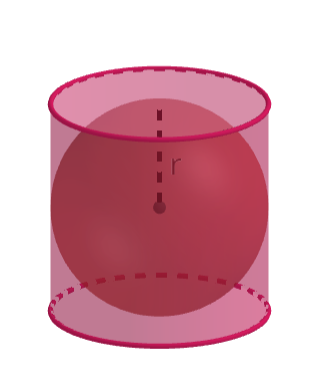
\includegraphics[width=.7\textwidth]{esfera_inscrita.png}
                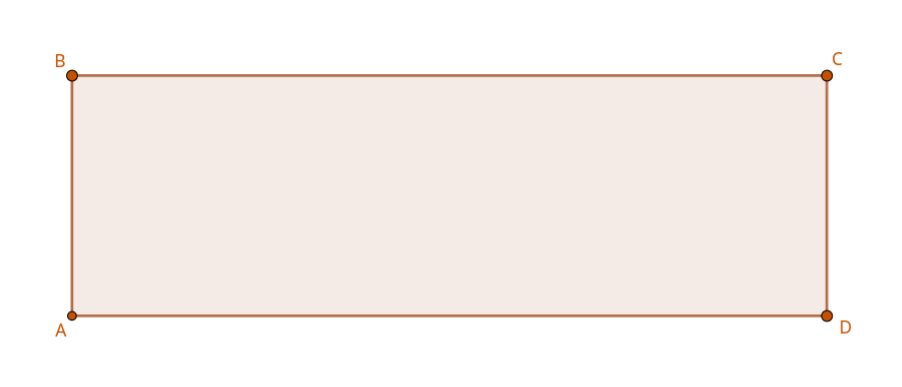
\includegraphics[width=.8\textwidth]{cilindro_planificacao_face.png}
            \end{column}
            \begin{column}{.38\textwidth}
                A área da superfície de uma esfera de raio $r$ é dada pela fórmula:
                
                {\Large
                \[
                    A = 4 \pi r^2
                \]
                }

                \vspace{1.2 em}

                Essa fórmula também foi descoberta e demonstrada por Arquimedes, que mostrou que a área da superfície de uma esfera é igual à área lateral do cilindro circunscrito a ela.

                \vspace{2em}

                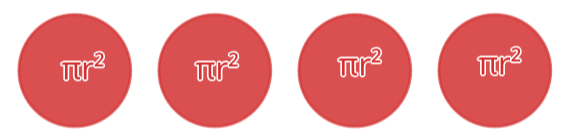
\includegraphics[width=\textwidth]{circulos.png}
            \end{column}
            
        \end{columns}
    \end{frame}

    \begin{frame}{Projeção Ortogonal}
        \begin{columns}[totalwidth=0.9\textwidth, T]
            \begin{column}{.3\textwidth}
                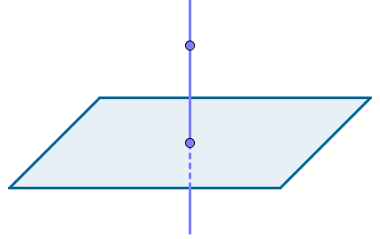
\includegraphics[width=.88\textwidth]{projecao_ponto.png}
                \vfill
                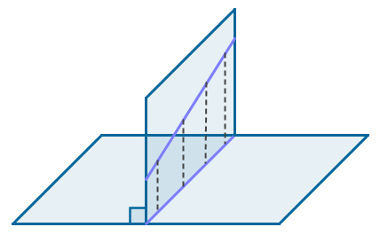
\includegraphics[width=.88\textwidth]{projecao_reta.png}
                \vfill
                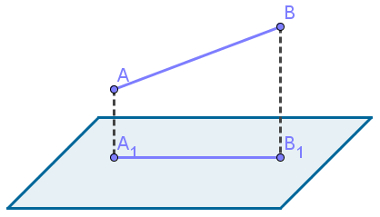
\includegraphics[width=.88\textwidth]{projecao_segmento.png}
            \end{column}
            \begin{column}{.6\textwidth}
                Projeções ortogonais são representações bidimensionais de objetos tridimensionais, obtidas projetando os pontos do objeto em um plano de projeção.

                \vspace{1.2em}

                Podemos entender a projeção ortogonal como a sombra de um objeto, quando iluminado por uma fonte de luz que emite raios paralelos, em ângulo reto.

                \vspace{1.2em}

                \begin{itemize}
                    \item A projeção ortogonal de um ponto é outro ponto;
                    \item A projeção ortogonal de uma reta é outra reta ou um ponto;
                    \item A projeção ortogonal de um segmento de reta é outro segmento de reta ou um ponto.
                \end{itemize}

                \vspace{1.2em}

                Retas e segmentos de reta que são ortogonais ao plano de projeção serão projetados em um ponto.
            \end{column}
        \end{columns}    
    \end{frame}

    \begin{frame}{Projeção Ortogonal de Figuras}
        \begin{columns}[totalwidth=.9\textwidth, T]
            \begin{column}{.6\textwidth}
                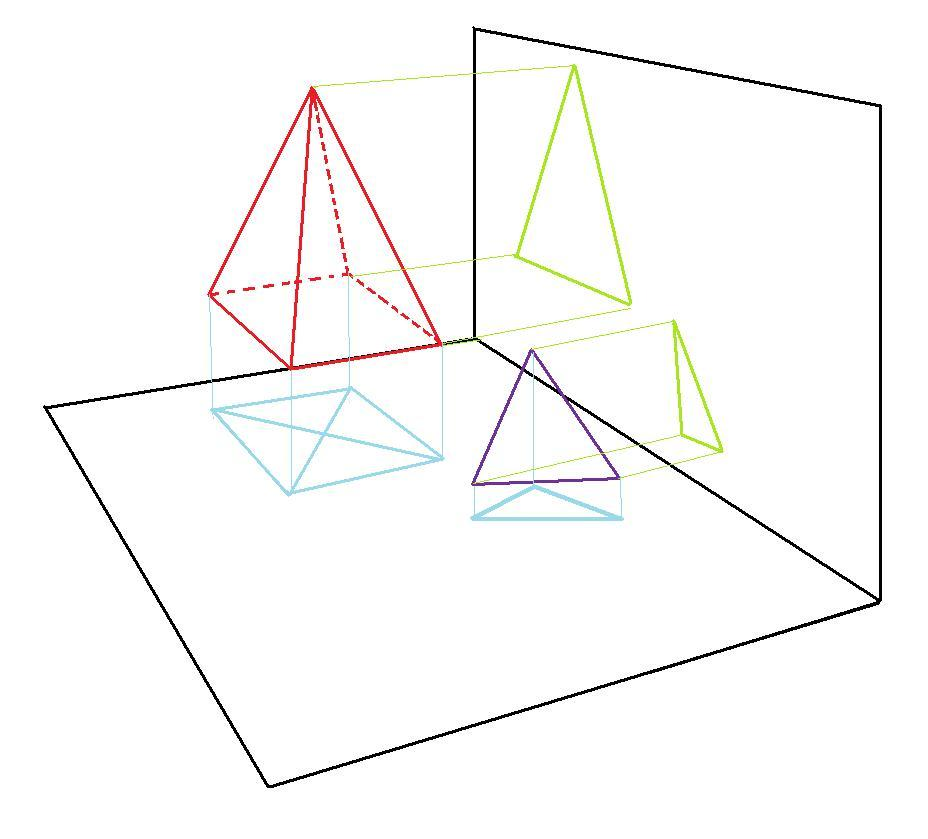
\includegraphics[width=.85\textwidth]{projecao_ortogonal.png}
            \end{column}

            \begin{column}{.38\textwidth}
                A projeção ortogonal de uma figura plana é outra figura plana. É o resultado da projeção de todos os seus pontos no plano de projeção.

                \vspace{1.2em}

                É preciso uma boa dose de imaginação para visualizar o resultado. No caso em que a projeção envolve figuras, tente pensar na projeção da sombra da figura ao sol do meio dia, ou da visualização de seus pontos-chaves sobre o plano.
            \end{column}
        \end{columns}
    \end{frame}
%----------------------------------------------
%              EXERCÍCIOS
%----------------------------------------------

    \begin{frame} {Exercícios} %Gabarito 1-C
        \begin{columns}
            \centering
            \begin{column}{.9\textwidth} %letra a
                1.~\textbf{(ENEM-2017): }Para decorar uma mesa de festa infantil, um chefe de cozinha usará um melão esférico com diâmetro medindo 10 cm, o qual servirá de suporte para espetar diversos doces. Ele irá retirar uma calota esférica do melão, conforme ilustra a figura, e, para garantir a estabilidade deste suporte, dificultando que o melão role sobre a mesa, o chefe fará o corte de modo que o raio r da seção circular de corte seja de pelo menos 3 cm. Por outro lado, o chefe desejará dispor da maior área possível da região em que serão afixados os doces.
            \vspace{1em}
            \begin{columns}[T]
                \centering
                \begin{column}{.55\textwidth}
                    \begin{figure}
                        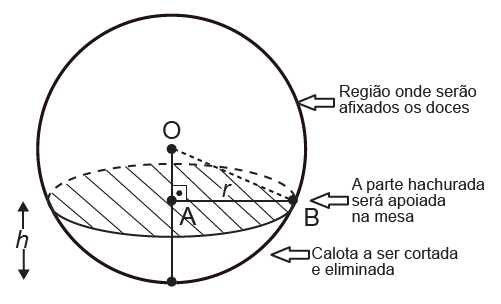
\includegraphics[width=.85\textwidth]{questao01.png}
                    \end{figure}
                \end{column}
                \begin{column}{.45\textwidth}
                    Para atingir todos os seus objetivos, o chefe deverá cortar a calota do melão numa altura h, em centímetro, igual a


                    \begin{enumerate}[label=\alph*)]
                        \item $\displaystyle 5 - \frac{\sqrt{91}}{2}$
                        \item $\displaystyle 10 - \sqrt{91}$
                        \item 1
                        \item 4
                        \item 5
                    \end{enumerate}
                \end{column}
            \end{columns}
            \end{column}    
        \end{columns}
    \end{frame}

    \begin{frame} {Exercícios} %Gabarito 2-B
        \begin{columns}[totalwidth=.9\textwidth]
            \begin{column}{\textwidth}
                2.\textbf{(ENEM-2013) } Gangorra é um brinquedo que consiste de uma tábua longa e estreita equilibrada e fixada em seu ponto central (pivô). Nesse brinquedo, duas pessoas sentam-se nas extremidades e, alternadamente, impulsionam-se para cima, fazendo descer a extremidade oposta, realizando assim o movimento da gangorra. Considere a gangorra representada na figura, em que os pontos A e B são equidistantes do pivô:
            \end{column}
        \end{columns}
        \vspace{1.8em}
        \begin{columns}[totalwidth=.9\textwidth, T]
            \begin{column}{.45\textwidth}
                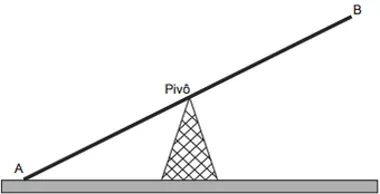
\includegraphics[width=\textwidth]{questao02.jpg}
            \end{column}

            \begin{column}{.45\textwidth}
                \centering
                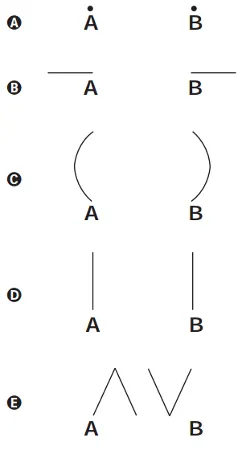
\includegraphics[width=.4\textwidth]{questao02_alternativas.jpg}
            \end{column}
        \end{columns}
    \end{frame}

    \begin{frame}{Exercícios} %Gabartito 3-C
        \begin{columns}[totalwidth=0.9\textwidth]
            \begin{column}{\textwidth}
                3. \textbf{(ENEM-2024) }Em um jogo virtual para celular, um personagem pode percorrer trajetórias retilíneas voando ou se deslocando ao longo de paredes. Considere que o personagem descreve a trajetória ABCDEF, em que os pontos A, D e E estão em um plano paralelo ao que contém os pontos B e C, sendo esses dois planos ortogonais ao plano da base que contém o ponto F, conforme a figura. A projeção ortogonal, sobre o plano da base, da trajetória ABCDEF descrita pelo personagem é
            \end{column}
        \end{columns}

        \vspace{1.8em}

        \begin{columns}[totalwidth=0.9\textwidth, T]
            \begin{column}{.45\textwidth}
                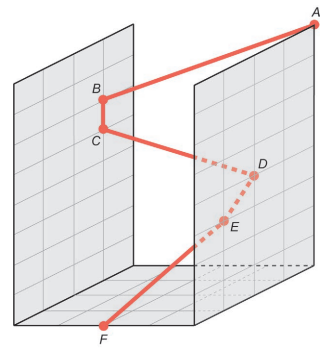
\includegraphics[width=.7\textwidth]{questao03.png}
            \end{column}

            \begin{column}{.45\textwidth}
                \centering
                \begin{tabular}{c c c}
                    {\bf a.} 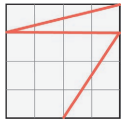
\includegraphics[width=.3\textwidth]{questao03-A.png} &
                    {\bf b.} 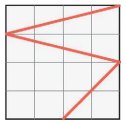
\includegraphics[width=.3\textwidth]{questao03-B.png} &
                    {\bf c.} 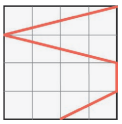
\includegraphics[width=.3\textwidth]{questao03-C.png}\\
                    \\
                    {\bf d.} 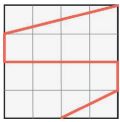
\includegraphics[width=.3\textwidth]{questao03-D.png} &
                    {\bf e.} 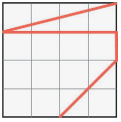
\includegraphics[width=.3\textwidth]{questao03-E.png} &
                \end{tabular}
            \end{column}
        \end{columns}
    \end{frame}

    \begin{frame}{Exercícios} %Gabarito 4-A
        \begin{columns}[totalwidth=.9\textwidth]
            \begin{column}{\textwidth}
                4. \textbf{(ENEM- 2010) }Se pudéssemos reunir em esferas toda a água do planeta, os diâmetros delas seriam:
            \end{column}
        \end{columns}

        \vspace{1.2em}

        \begin{columns}[totalwidth=.9\textwidth, T]
            \begin{column}{.45\textwidth}
                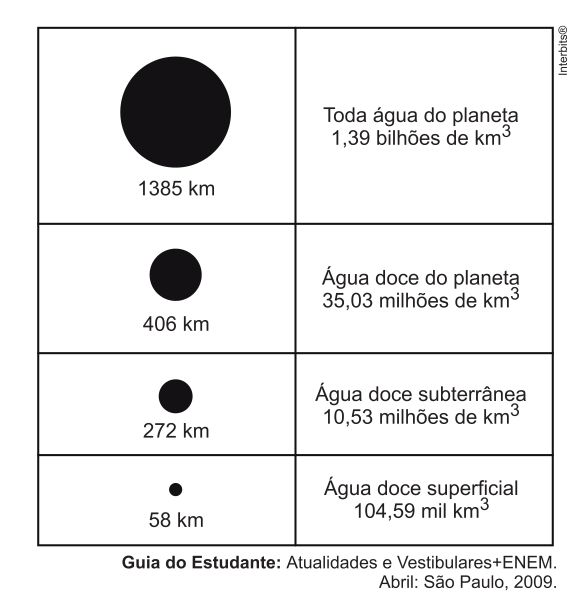
\includegraphics[width=.9\textwidth]{questao04.png}
            \end{column}
            \begin{column}{.45\textwidth}
                A razão entre o volume da esfera que corresponde à água doce superficial e o volume da esfera que corresponde à água doce do planeta é

                \vspace{0.8em}

                \begin{enumerate}[label=\alph*)]
                    \item $\displaystyle\frac{1}{343}$ \vspace{0.8em}
                    \item $\displaystyle\frac{1}{49}$ \vspace{0.8em}
                    \item $\displaystyle\frac{1}{7}$ \vspace{0.8em}
                    \item $\displaystyle\frac{29}{136}$ \vspace{0.8em}
                    \item $\displaystyle\frac{136}{203}$ \vspace{0.8em}
                \end{enumerate}
            \end{column}
        \end{columns}
    \end{frame}

    \begin{frame}{Exercícios} %Gabarito 5-E
        \begin{columns}[totalwidth=.9\textwidth]
            \begin{column}{\textwidth}
                5. \textbf{(Espcex(AMAN)-2018) } A angioplastia é um procedimento médico caracterizado pela inserção de um cateter em uma veia ou artéria com o enchimento de um pequeno balão esférico localizado na ponta desse cateter. Considerando que, num procedimento de angioplastia, o raio inicial do balão seja desprezível e aumente a uma taxa constante de $0,5$ mm/s até que o volume seja igual a $500\text{ mm}^3$, então o tempo, em segundos, que o balão leva para atingir esse volume é
                
                \vspace{1.2em}

                \begin{enumerate}[label=\alph*)]
                    \item $10$ \vspace{.3em}
                    \item $\displaystyle 10 \sqrt[3]{\frac{5}{\pi}}$ \vspace{.3em}
                    \item $\displaystyle 10 \sqrt[3]{\frac{2}{\pi}}$ \vspace{.3em}
                    \item $\displaystyle 10 \sqrt[3]{\pi}$ \vspace{.3em}
                    \item $\displaystyle 10 \sqrt[3]{\frac{3}{\pi}}$
                \end{enumerate}
            \end{column}
        \end{columns}
    \end{frame}

    % \begin{frame} {Exercícios} %Gabarito 3-D
    %     \begin{columns}[totalwidth=.9\textwidth]
    %         \begin{column}{\textwidth}
    %             3 \textbf{(ENEM-2010) }Uma fábrica de tubos acondiciona tubos cilíndricos menores dentro de outros tubos cilíndricos. A figura mostra uma situação em que quatro tubos cilíndricos estão acondicionados perfeitamente em um tubo com raio maior

    %             \vspace{1em}
                
    %             Uma fábrica de tubos acondiciona tubos cilíndricos menores dentro de outros tubos cilíndricos. A figura mostra uma situação em que quatro tubos cilíndricos estão acondicionados perfeitamente em um tubo com raio maior
    %         \end{column}   
    %     \end{columns}
    %         \vspace{1.8em}

    %     \begin{center}
    %         \begin{columns}
    %             \begin{column}{.4\textwidth}
    %                 \begin{figure}
    %                     \includegraphics[width=.7\textwidth]{questao_03.png}
    %                 \end{figure}
    %             \end{column}
    %             \hfill
    %             \begin{column}{.5\textwidth}
    %                 \begin{enumerate}[a. ]
    %                     \item $12 \text{ cm}$
    %                     \item $12 \sqrt{2}\text{ cm}$
    %                     \item $24 \sqrt{2}\text{ cm}$
    %                     \item $6 \left( 1 + \sqrt{2}\right) \text{ cm}$
    %                     \item $12 \left( 1 + \sqrt{2}\right) \text{ cm}$
    %                 \end{enumerate}
    %             \end{column}
    %         \end{columns}
    %     \end{center}
    % \end{frame}

    % \begin{frame} {Exercícios} %Gabarito 4-A
    %     \begin{columns}[totalwidth=.9\textwidth]
    %         \begin{column}{\textwidth}
    %             4 \textbf{(UNICAMP-2011) }Depois de encher de areia um molde cilíndrico, uma criança virou-o sobre uma superfície horizontal. Após a retirada do molde, a areia escorreu, formando um cone cuja base tinha raio igual ao dobro do raio da base do cilindro.
    %         \end{column}   
    %     \end{columns}
    %         \vspace{1.8em}

    %     \begin{center}
    %         \begin{columns}[totalwidth=.9\textwidth, T]
    %             \begin{column}{.4\textwidth}
    %                 \includegraphics[width=.9\textwidth]{questao_04.png}
    %             \end{column}

    %             \begin{column}{.45\textwidth}
    %                 A altura do cone formado pela areia era igual a

    %                 \vspace{1.2em}

    %                 \begin{enumerate}[a. ]
    %                     \item $\displaystyle\frac{3}{4}$ da altura do cilindro.\vspace{0.8em}
    %                     \item $\displaystyle\frac{1}{2}$ da altura do cilindro.\vspace{0.8em}
    %                     \item $\displaystyle\frac{2}{3}$ da altura do cilindro.\vspace{0.8em}
    %                     \item $\displaystyle\frac{3}{1}$ da altura do cilindro.\vspace{0.8em}
    %                 \end{enumerate}
    %             \end{column}
    %         \end{columns}
    %     \end{center}
    % \end{frame}

    % \begin{frame} {Exercícios} %Gabarito 5-A
    %     \begin{columns}[totalwidth=.9\textwidth]
    %         \begin{column}{\textwidth}
    %             5 \textbf{(ENEM-2020) }Num recipiente com a forma de paralelepípedo reto-retângulo, colocou-se água até a altura de 8 cm e um objeto, que ficou flutuando na superfície da água.  
                
    %             Para retirar o objeto de dentro do recipiente, a altura da coluna de água deve ser de, pelo menos, 15 cm. Para a coluna de água chegar até essa altura, é necessário colocar dentro do recipiente bolinhas de volume igual a $6\text{ cm}^3$ cada, que ficarão totalmente submersas. 
    %         \end{column}
    %     \end{columns}

    %     \vspace{1.3em}
        
    %     \begin{columns}[totalwidth=.95\textwidth, T]
    %         \begin{column}{.3\textwidth}
    %             \begin{figure}
    %                 \centering
    %                 \includegraphics[width=\textwidth]{questao_05.png}
    %             \end{figure}
    %         \end{column}

    %         \hfill

    %         \begin{column}{.6\textwidth}
    %             O número mínimo de bolinhas necessárias para que se possa retirar o objeto que flutua na água, seguindo as instruções dadas, é de

    %             \vspace{1.2em}

    %             \begin{enumerate}[a. ]
    %                 \item 14.
    %                 \item 16.
    %                 \item 18.
    %                 \item 30.
    %                 \item 34.
    %             \end{enumerate}
    %         \end{column}
    %     \end{columns}
    % \end{frame}

\end{document}